\documentclass[12pt]{article}

\usepackage[brazilian]{babel}
\usepackage[utf8]{inputenc}
\usepackage[T1]{fontenc}
\usepackage{graphicx}
\everymath{\displaystyle}
\usepackage{amssymb}



\begin{document}
\date{}
\title{2ª PROVA DE CÁLCULO}
\author{Prof. Renato Vidal da Silva Martins}
\maketitle

\part{Enunciados}
\begin{enumerate}
	\item Calcule os limites:
	\begin{enumerate}
		\item (4 pontos) $ \lim\limits_{x \rightarrow 0}x^2 cossec(3x) $
		\item (4 pontos) $ \lim\limits_{x \rightarrow 0^{+}} (\sin(x))^x $
	\end{enumerate}
	\item (8 pontos) Um cone de $1 cm$ de raio, $2 cm$ de altura está cheio de água. Fazendo um furo no bico, começa a vazar a uma taxa de $\pi/4$ $cm^3/s$. Calcule a taxa de variação do nível de água no instante em que 7/8 do volume já vazou.\\Volume do cone: $\frac{\pi r^2 h}{3}$
	\item (9 pontos) Esboce o gráfico da função
	\begin{center}
		$ f(x) =  -xe^x$
	\end{center}
	
	determinando: domínio, interceptos com os eixos coordenados, análise de sinal da função, limites pertinentes, crescimento e decrescimento, concavidade.
	\item (8 pontos) As margens superior e inferior de um cartaz retangular devem medir $6cm$ cada e as margens esquerda e direita devem pedir $4cm$ cada. O texto deve ocupar uma área de $384cm^2$. Encontre as dimensões do cartaz de menor área que satisfaça os requisitos acima.
\end{enumerate}

\newpage
\part{Resolução}
\begin{enumerate}
	\item Calcule os limites:
	\begin{enumerate}
		\item (4 pontos) $ \lim\limits_{x \rightarrow 0}x^2 cossec(3x) $
		\\
		Notamos uma indeterminação do tipo $0.\infty$, então prosseguimos tentando melhorar a expressão:
		\begin{center}
			$ \lim\limits_{x \rightarrow 0}x^2 cossec(3x) =$ \\
			$ \lim\limits_{x \rightarrow 0}\frac{x^2}{\sin(3x)} =$\\
			$ \lim\limits_{x \rightarrow 0}\frac{3}{3} . \frac{x^2}{\sin(3x)} =$\\
			$ \lim\limits_{x \rightarrow 0}\frac{3x^2}{3 \sin(3x)} =$\\
			$ \lim\limits_{x \rightarrow 0}\left(  \frac{3 \sin(3x)}{3x^2} \right) ^{-1} =$\\
			$ \lim\limits_{x \rightarrow 0}\left(  \frac{3}{x} \right) ^{-1} =$\\
			$ \lim\limits_{x \rightarrow 0}\frac{x}{3}= 0$\\
		\end{center}
		
		\item (4 pontos) $ \lim\limits_{x \rightarrow 0^{+}} (\sin(x))^x $
		\\
		Como sabemos que estamos tentando a zero pelo lado positivo podemos dizer que $k^x$ tende a 1, como o seno é uma função limitada entre -1 e 1 podemos dizer que:
		\begin{center}
			$ \lim\limits_{x \rightarrow 0^{+}} (-1)^x \le  \lim\limits_{x \rightarrow 0^{+}} (\sin(x))^x \le \lim\limits_{x \rightarrow 0^{+}} (1)^x$\\
			$ 1 \le  \lim\limits_{x \rightarrow 0^{+}} (\sin(x))^x \le 1$\\
			$ \lim\limits_{x \rightarrow 0^{+}} (\sin(x))^x = 1$\\
		\end{center}
		
	\end{enumerate}
	\item (8 pontos) Um cone de $1 cm$ de raio, $2 cm$ de altura está cheio de água. Fazendo um furo no bico, começa a vazar a uma taxa de $\pi/4$ $cm^3/s$. Calcule a taxa de variação do nível de água no instante em que 7/8 do volume já vazou.\\Volume do cone: $\frac{\pi r^2 h}{3}$\\
	\\
	O exercício pede a taxa de variação do nível da água no instante em que restam 1/8 do conteúdo original, para tanto é preciso escrever a função que fornece a altura em função do volume dado.\\
	Observando a formula do volume e tendo em mente semelhança de triângulos podemos notar que quando a altura é reduzida a uma porcentagem $x$ o volume todo é reduzido a uma porcentagem $x^3$ do original. Ou seja:\\
	
	\begin{center}
		$ Volume_{atual} = \left( \frac{Altura_{atual}}{Altura_{inicial}} \right)^3 \times Volume_{inicial} $\\
		$ Volume_{atual} = Volume_{inicial} - \frac{\pi t}{4} = \frac{8\pi - 3\pi t}{12}$\\
		$ Altura_{atual} = Altura_{inicial} \sqrt[3]{\frac{Volume_{atual} }{Volume_{inicial} } }$\\
		
		$ h(V) = h_{0} \sqrt[3]{\frac{V}{V_{0} } } = 2\sqrt[3]{\frac{3V}{2\pi}}   $\\
		
		$ h(t) = 2 \sqrt[3]{\frac{8 - 3t}{8} }$\\
	\end{center}
	
	Para calcular o volume inicial basta tomar a fórmula:
	
	\begin{center}
		$\frac{\pi r^2 h}{3} = \frac{\pi 1^2.2}{3} = \frac{2\pi}{3}$
	\end{center}
	
	O volume que queremos localizar é:
	
	\begin{center}
		$\frac{1}{8}.\frac{2\pi}{3} = \frac{\pi}{12}$
	\end{center}
	
	A taxa de variação da altura em um momento é a sua derivada, então:
	
	\begin{center}
		$ \left[ 2 \sqrt[3]{\frac{8 - 3t}{8}} \right] ' = -\frac{1}{4} \left( \frac{8}{8-3t}\right) ^{\frac{2}{3}} $\\
	\end{center}
	
	Vamos descobrir o tempo igualando na equação do volume em função do tempo:
	
	\begin{center}
		$ \frac{\pi}{12} = \frac{8\pi - 3\pi t}{12}$\\
		$ t = \frac{7}{3}$\\
	\end{center}
	
	Substituindo no ponto teremos:
	
	\begin{center}
		$ -\frac{1}{4} \left( \frac{8}{8-3 \times \frac{7}{3}}\right) ^{\frac{2}{3}} = -1$\\
	\end{center}
	
	Então a taxa de variação no instante requerido é de $-1 cm/s$.
	
	\begin{center}
		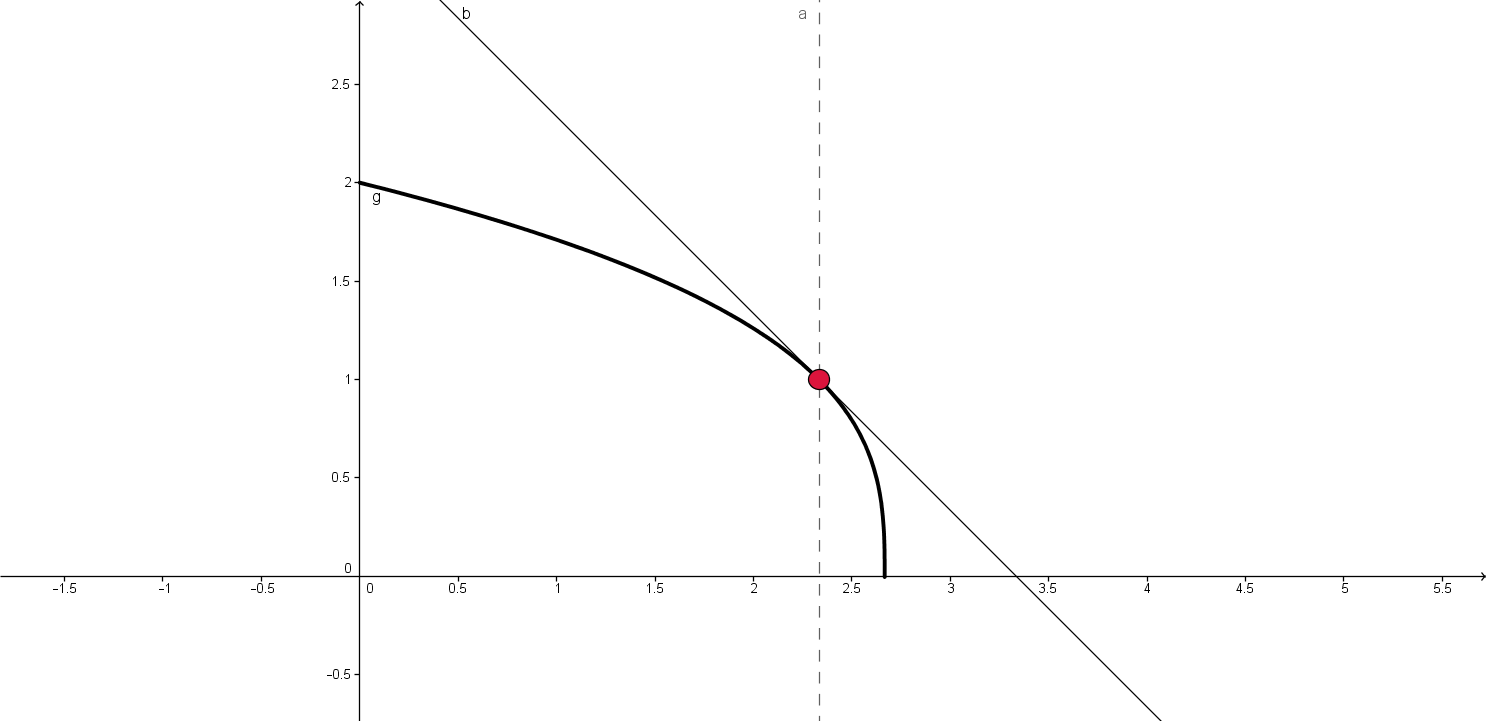
\includegraphics{img/volume.png}
	\end{center}
	
	Observe que a variação é negativa, confirmando a ideia de que o nível da água reduz quando ela vai esvaziando. E observando o gráfico podemos observar ainda que ele reduz mais rapidamente quanto menor o volume restante.
	\\	
	
	\item (9 pontos) Esboce o gráfico da função
	\begin{center}
		$ f(x) =  -xe^x$
	\end{center}
	
	determinando: domínio, interceptos com os eixos coordenados, análise de sinal da função, limites pertinentes, crescimento e decrescimento, concavidade.\\
	\\
	Analisando o domínio das duas funções separadamente percebemos que ambas são válidas no domínio dos reais, já que $-x$ e $e^x$ são válidos para qualquer $x$.\\
	Os interceptos com os eixos acontecem quando $x=0$ ou $y=0$, então basta calcular:
	\begin{center}
		$ y =  -xe^x$\\
		$ 0 =  -xe^x \rightarrow x = 0 \rightarrow P_1(0,0) $\\
		$ y =  -0.e^0 \rightarrow y = 0 \rightarrow P_2(0,0) $
	\end{center}
	Notamos que só existem interceptos com os eixos na origem.
	\\
	Analisando o sinal de $e^x$ percebemos que ele sempre será positivo, logo o sinal da função $-xe^x$ é determinado pelo valor de x. Quando x é positivo então a função tem sinal negativo e quando x é negativo a função tem sinal positivo.
	\\
	Vamos analisar $-xe^x$ para $x<0$. Tomando x = |x|, podemos escrever $\frac{x}{e^x}$, já para $x>0$ a tomando x = |x| temos $-xe^x$. Note que no $x<0$ a função possui um limite que é zero, já com $x>0$ não existem limites pertinentes.
	\\
	Para encontrar os pontos de crescimento e decrescimento precisamos encontrar a primeira derivada:
	\begin{center}
		$ \left[ -xe^x \right] ' =  -e^x-xe^x $
	\end{center}
	Quando ela for maior que zero haverá crescimento, quando for menor que zero decrescimento, então:
	\begin{center}
		$ -e^x-xe^x > 0 \rightarrow x < -1$\\
		$ -e^x-xe^x > 0 \rightarrow x > -1$
	\end{center}
	Ou seja, ela é crescente para $x<-1$, decrescente para $x>-1$, e seu ponto de inflexão está localizado em $x=-1$.
	\\
	Para obter a concavidade precisamos da segunda derivada:
	\begin{center}
		$ \left[ -xe^x \right] '' =  \left[ -e^x-xe^x \right] ' = -2e^x-xe^x $
	\end{center}
	Quando a segunda derivada é positiva a concavidade é para cima, quando é negativa a concavidade é para baixo, logo:
	\begin{center}
		$ -2e^x-xe^x > 0 \rightarrow x < -2$\\
		$ -2e^x-xe^x > 0 \rightarrow x > -2$
	\end{center}
	A função é concava para cima com $x<-2$ e para baixo com $x>-2$.\\
	Com esses dados podemos finalmente desenhar o gráfico da função como abaixo.
	\begin{center}
		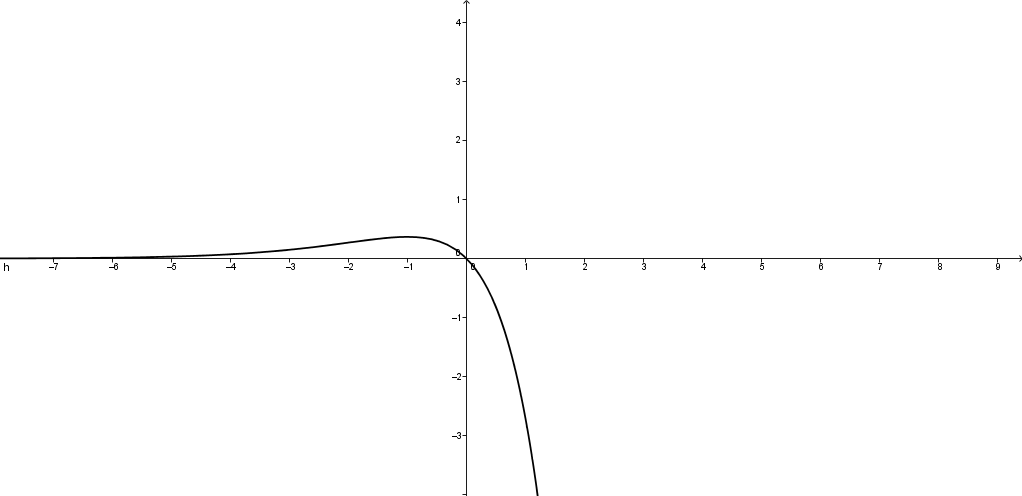
\includegraphics{img/func.png}
	\end{center}
	
	
	\item (8 pontos) As margens superior e inferior de um cartaz retangular devem medir $6cm$ cada e as margens esquerda e direita devem pedir $4cm$ cada. O texto deve ocupar uma área de $384cm^2$. Encontre as dimensões do cartaz de menor área que satisfaça os requisitos acima.
	\\
	\\
	Vamos considerar que a área total é $xy$, então $(x-12)(y-8)=384$, desenvolvendo:
	\begin{center}
		$(x-12)(y-8)=384$\\
		$y= \frac{8x+288}{x-12}$
	\end{center}
	A área é, portanto:
	\begin{center}
		$A(x) = x\frac{8x+288}{x-12}$
	\end{center}
	Para obter a menor área temos que encontrar os pontos de máximo e mínimo, ou seja, quando a primeira derivada se iguala a zero:
	\begin{center}
		$\left[  x\frac{8x+288}{x-12} \right]' = \frac{(16x+288)(x-12)-(1)(8x^2+288x)}{(x-12)^2}$\\
		
		$ \frac{(16x+288)(x-12)-(1)(8x^2+288x)}{(x-12)^2} = 0 \rightarrow x = 36$ ou $x = -12$\\
	\end{center}
	Como $-12$ não é um valor válido para comprimento vamos considerar $x=36$, calculando temos $y=24$, então o cartaz possui dimensões $24x36$.
	
\end{enumerate}


\end{document}